
\documentclass{mcmthesis}
\mcmsetup{CTeX = false,   % 使用 CTeX 套装时,设置为 true
        tcn = 1920682, problem = B,
        sheet = true, titleinsheet = true, keywordsinsheet = true,
        titlepage = true}
\usepackage{amsmath, amssymb}
\usepackage{mathrsfs}
\usepackage{palatino}
\usepackage{mwe}
\usepackage{graphicx}
\usepackage{subfig}
\usepackage{subcaption}
\usepackage{float}
\usepackage{multirow}
\usepackage{indentfirst}
\usepackage{gensymb}
\usepackage[ruled,lined,commentsnumbered]{algorithm2e}
\usepackage{geometry}
\usepackage{pdfpages}
\usepackage{array}
\usepackage{verbatim}
\usepackage{algorithm}
\geometry{left=2cm,right=2cm,top=2cm,bottom=2cm} %%页边距
\begin{document}
\linespread{0.6} %%行间距
\setlength{\parskip}{0.5\baselineskip} %%段间距

\section{Statement of Our Model}
\subsection{Route Selection Model}
\subsubsection{Delivery-Prioritized Region}
Now we shift our attention to the delivery-prioritized region, which refers to the north central part on the island. We call this place \emph{delivery-prioritized} because we have to serve three of the five hospitals in this region. In this place, the efficiency of transporting medical packages to hospitals is the top priority, while the video reconnaissance work should not be ignored. With this situation in consideration, we first propose a strategy for each drone in the container to load medical packages into its bay and transport to a certain hospital. Then the drone can decide its path of returning back, which maximizes road coverage.

When a drone is about to take off, the content of the bay tied to a drone taking off must be decided. Here we can randomly choose a packaging strategy that satisfies the payload capabilities of the drone. The packaging strategy candidates are already provided in Container Internal Placement Model. The best combination of packaging strategies for all drones can be later figured out by a heuristic algorithm.

As demonstrated in Destination Selection Model, the location of the container in delivery-prioritized region is chosen in such a way that the drone of both type deployed, i.e. Drone B and Drone C, can reach any of the hospital in delivery-prioritized region and return safely. After the bay is packaged, a drone randomly choose a hospital in this region. The best distribution of the drone flow can also be figured out by a heuristic algorithm.

After delivering the medical packages, the drone has to return to container and wait for charging. Since the drone has completed its major task, the efficiency of video reconnaissance should be considered. If the drone returns in straight line, the margin of the battery life may not be fulled exploited to assess major roads. However, as the power is not so efficient, the returning route cannot be too twisted, in which case the drone may have difficulty reaching container. 

Here we use \textbf{Quadratic B\'{e}zier Curve} to depict this returning route. B\'{e}zier Curve is widely used in many fields, such as computer graphics and robotics. The $n$th order of B\'{e}zier Curve is determined by $n+1$ points $P_0, P_1, ..., P_{n}$. A Quadratic B\'{e}zier Curve can be expressed mathematically as:
\begin{equation}
    \mathbf{B}(t)=(1-t)^2\mathbf{P}_0 + 2(1-t)\mathbf{P}_1 + t^2\mathbf{P}_2, 0 \leq t \leq 1
    \label{Equ:bezr}
\end{equation}

\begin{figure}[htbp]
    \centering
    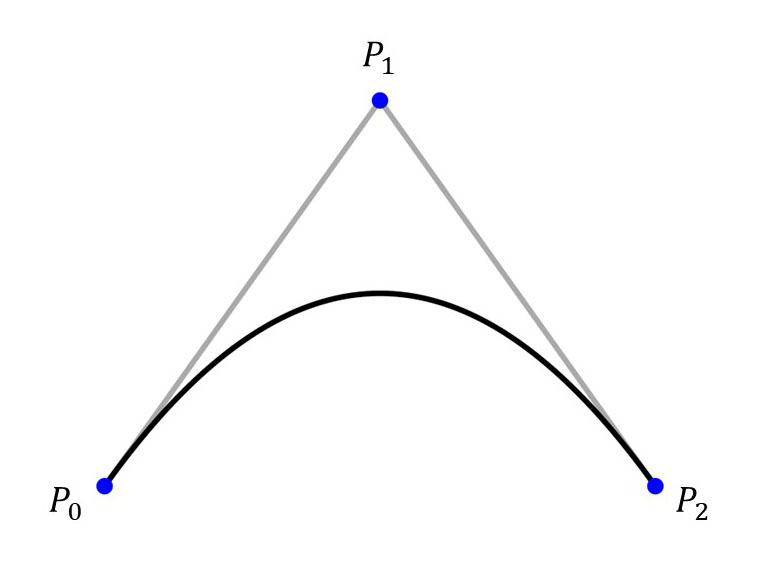
\includegraphics[width=10cm,height=6cm]{figures/bezier.jpg}
    \caption{Plot of Quadratic B\'{e}zier Curve}
    \label{Fig:bezr}
\end{figure}

A plot of Quadratic B\'{e}zier Curve is shown in Figure \ref{Fig:bezr}. Higher orders of B\'{e}zier Curve are also available, but need more control points and may look more twisted. That's why we choose the quadratic one. 

The length of a B\'{e}zier Curve can be expressed by the following integral:
\begin{equation}
\begin{aligned}
    |\mathbf{B}| &= \int_B \mathrm{d}l = \int_0^1 \sqrt{[P_x'(t)]^2 + [P_y'(t)]^2} \mathrm{d}t \\
    &= \int_0^1 2\sqrt{[-(1-t)P_{0x}+(1-2t)P_{1x}+tP_{2x}]^2 + [-(1-t)P_{0y}+(1-2t)P_{1y}+tP_{2y}]^2} \mathrm{d}t
\end{aligned}
\label{Equ:bezl}
\end{equation}
Note that this equation is rather difficult to get its analytic solution. In practice, we subdivide this curve into several line segments and compute the sum of their lengths. With Equation \ref{Equ:bezl}, we can get the length of a drone's returning route.

A drone has to assess road conditions in Puerto Rico, so a criterion must be defined to evaluate the effectiveness of video capture. First we consider a certain point on the route. Suppose a drone with field of view \cite{FieldOfView} $f$ is at height $h_D$, then the ground area covered by the camera can be approximated by a circle of radius $r_c = h_D \cdot f/2$. With this in mind, we can define road coverage of a route $\mathbf{B}$ as:
\begin{equation}
    C(\mathbf{B}) = \frac{w_r}{\pi r_c^2} \int_B\mathrm{d}l \iint_{S_t} I_R(x, y) \mathrm{d}x\mathrm{d}y
    \label{Equ:rtcv}
\end{equation}
where:
\begin{itemize}
    \item $w_r$ is the average width of road
    \item $S_t$ is the circle area centered at $\mathbf{B}$(t) with radius $r_f$
    \item $I_{R}(x, y)$ is the indicator function which indicates whether the point $(x, y)$ is on roads.
\end{itemize}

\begin{figure}[ht]
	\centering
	\begin{minipage}[t]{0.48\textwidth}
		\centering
		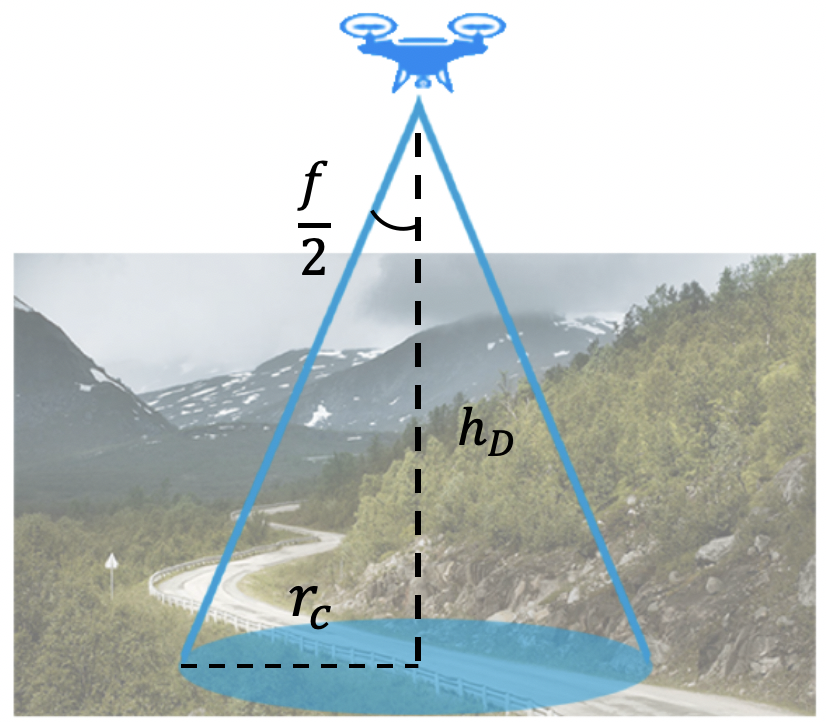
\includegraphics[width=8cm,height=7cm]{figures/fov.png}
		\centering{(a) Road Coverage on a Single Point}
	\end{minipage}
	\begin{minipage}[t]{0.48\textwidth}
		\centering
		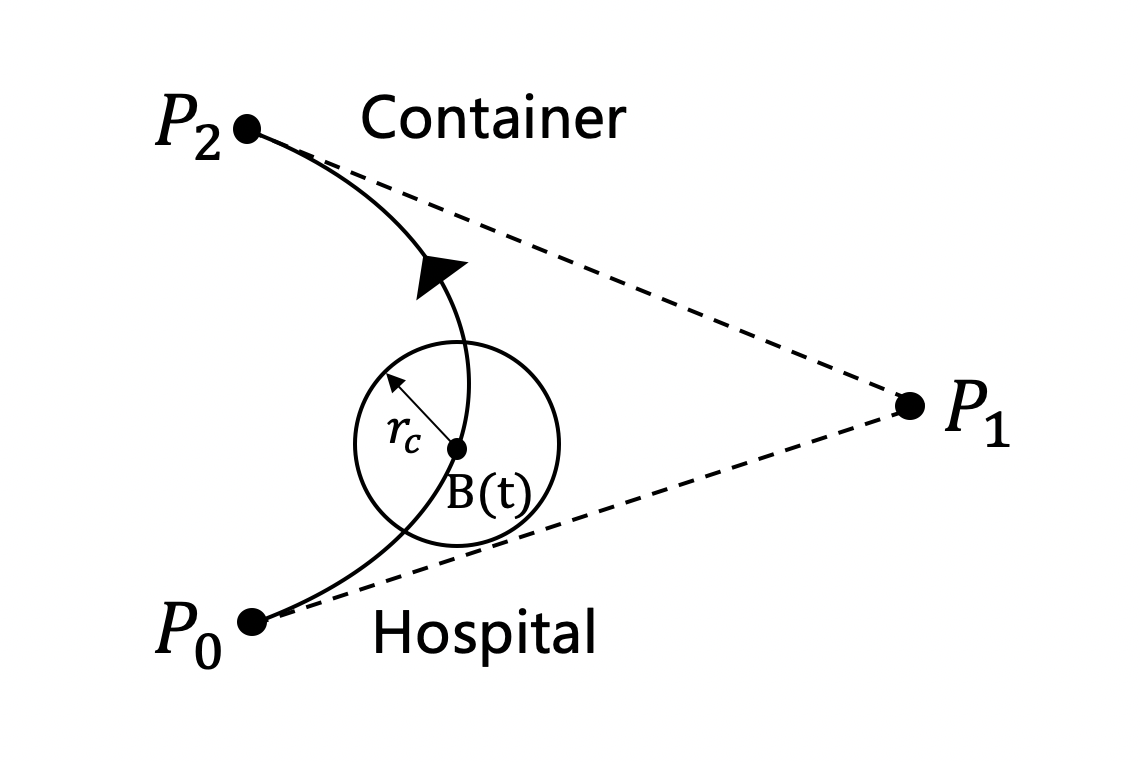
\includegraphics[width=8cm]{figures/route_coverage.png}
        \centering{(b) Road Coverage along a Returning Route}
	\end{minipage}
	\caption{Determination of Road Coverage}
	\label{Fig:rdcv}
\end{figure}

After defining the coverage $C(\mathbf{B})$, we have to find a way that can maximize road coverage on the returning route. Because of the difficulty of integrating over the whole curve, we resort to a local search method. We connect the hospital and container with a straight line segment $l_s$. Then we draw a line segment $l_p$ of length $2|l_s|$ which is perpendicular to $l_s$ and its midpoint coincides with the one of $l_s$. We divide $l_p$ into several segments, put B\'{e}zier Curve control point $P_1$ at each endpoint of these segments and try to find the position which has the largest $C(\mathbf{B})$. The method is demonstrated in Figure \ref{Fig:lcsr}.

\begin{figure}[htbp]
    \centering
    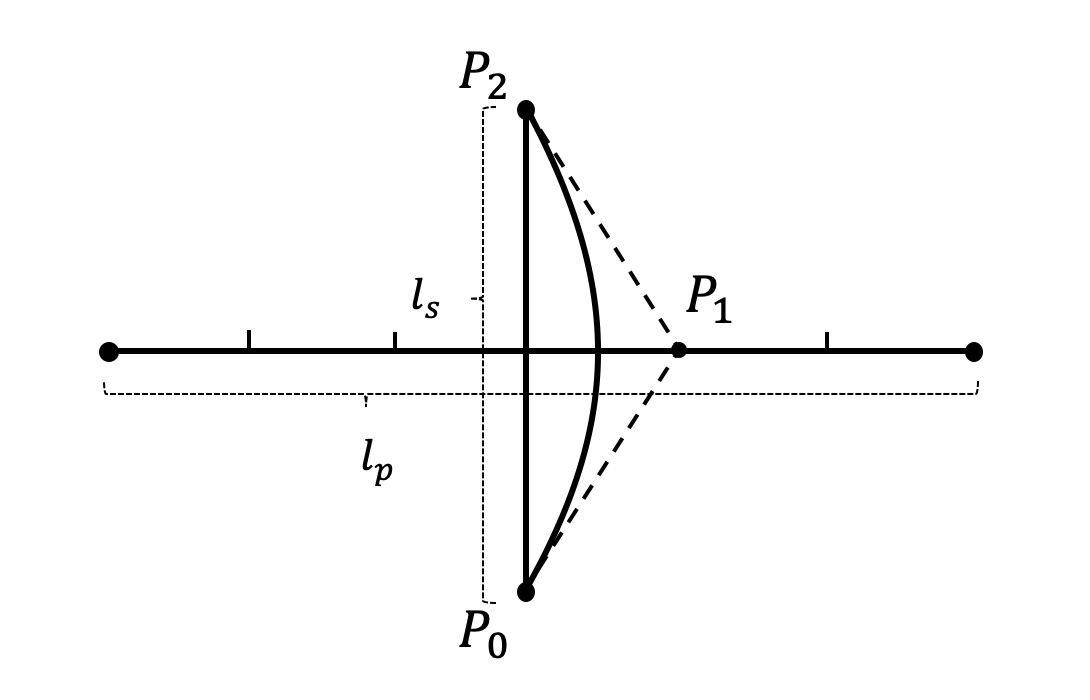
\includegraphics[width=10cm]{figures/local_search_route.png}
    \caption{Local Search of Best-Covering Route}
    \label{Fig:lcsr}
\end{figure}

\subsubsection{Reconnaissance-Prioritized Region}
In this part we discuss the other two regions: the one on the north-east coast and the one on the north-west cost. The two share in common that there is only one hospital in each of the region and the demand for medical packages are relatively low. In this region, the delivery is not so important as it is in delivery-prioritized one. More drones should be deployed to assess the roads instead of sending goods. The deployment strategy could be quite different from the one discussed in delivery-prioritized region.

Since the demand for goods is low, a small number of drones sending a fixed set of medical packages can sufficiently meet the demand. Therefore, no randomness is involved in this region and we don't need any heuristic algorithm to find an optimal solution. Among all the drones in the containers transported to these two locations, Drone F is only capable of delivering goods, so the two Drone F's should shoulder the responsibility of transporting medical packages. The bay packaging for Drone F's in these regions can specified explicitly, according to the demand of target hospitals. The other two types, Drone B and Drone C are assigned to assess nearby roads. 

For reconnaissance-oriented drones, the routes design should be different from the one discussed in previous part, in that it doesn't have to transport packages and should fully explore the roads nearby. The strategy is that when a drone takes off, it searches for the nearest road that has not been discovered and march to that point. It follows the roads and captures videos of them, while keeping track of the distance from the container and judging whether it should return, in case it may not be able to get back if battery life runs out. If the battery life could not support drone to cruise further, it returns to the container along the straight line route.

The situation gets complicated if we consider of the variable shapes of roads. In that way, the total road coverage of drones may be hard to expect. Here we firstly consider a simplified case, as shown in Figure \ref{Fig:vdsr} . Suppose there is a semi-infinite road. A container is away from the road by $d$. Drones are released from containers, one by one. The route of the first, second and third drone are marked on the figure. The furthest point on axis X on the road the $i$th drone can reach is denoted as $x_i$, and the length of road covered by the $i$th drone $l_i$. Therefore, we have $l_i=x_i-x_{i-1}$. Suppose the maximum length a drone can fly through is $s$, using Pythagorean theorem, we have:
\begin{equation}
    \sqrt{d^2+x_{i-1}^2} + l_i + \sqrt{d^2+x_i^2} = s
    \label{Equ:drvr}
\end{equation}
According to Equation \ref{Equ:drvr}, we can get the recursion formula of series $x_i$:
\begin{equation}
    \left\{
    \begin{aligned}
    &x_0 = 0 \\
    &x_i = \frac{(s + x_{i-1} - \sqrt{d^2 + x_{i-1}})^2 - d^2}{2(s + x_{i-1} - \sqrt{d^2 + x_{i-1}^2})}
    \end{aligned}
    \right.
\end{equation}

\begin{figure}[htbp]
    \centering
    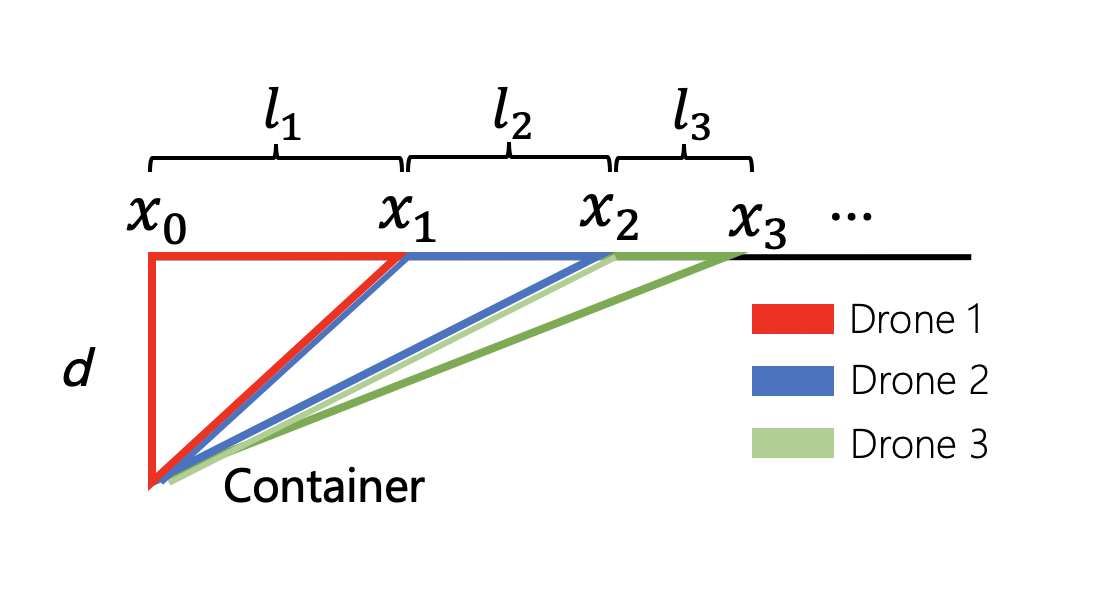
\includegraphics[width=10cm]{figures/video_drone_path.png}
    \caption{A Simplified Case of Drone Routes for Video Reconnaissance}
    \label{Fig:vdsr}
\end{figure}

We set $s$ to be the average flight distance of drones in the fleet, and $d$ to be average distance from the containers to the roads nearby. We compute the first several elements in the series and plot it on the graph. We find that this series can be fitted with an exponential function. See Figure \ref{Fig:cvft} for the plotted graph. We find that the the more drones we put into use, the less coverage a single drone can produce. That's because when more drones are launched, the farther the drone has to fly to reach the starting location of video capture. Since the battery life of a drone is fixed, the distance that a drone can actually spend on road assessment decreases continuously. 

The actual road condition may be far more complicated than the one discussed preciously, but we can infer that they have similar growing trend. So we can define the coverage function of the $i$th reconnaissance-prioritized region $C_i$ as the following:
\begin{equation}
    C_i = S_i(1 - e^{-\alpha N_{D,i}})
\end{equation}
where 
\begin{itemize}
    \item $S_i$ is the road area that is reachable by drones with straight line routes in the $i$th reconnaissance-prioritized region. 
    \item $N_{D,i}$ is the number of drones assigned to carry out video reconnaissance work 
\end{itemize}
In our implementation, we set $\alpha$ to be 1.7293. The sensitivity analysis of this parameter is discussed in the next section.

\begin{figure}[htbp]
    \centering
    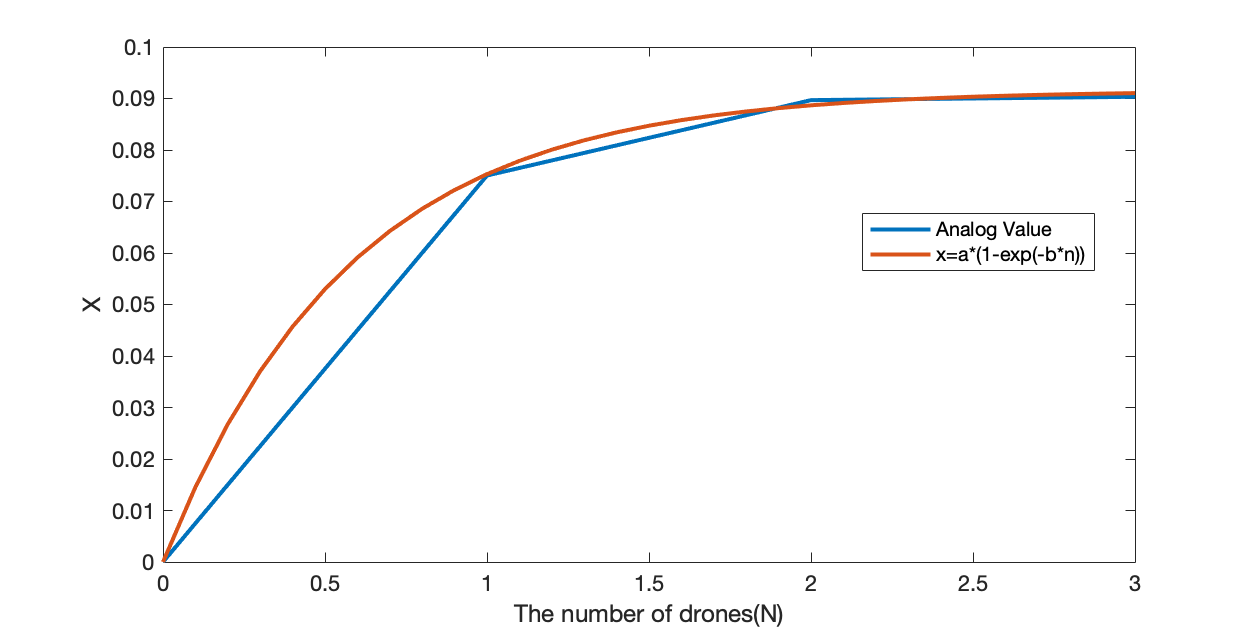
\includegraphics[width=12cm,height=6cm]{figures/alpha6.png}
    \caption{Plot of the Series and Fitting Function}
    \label{Fig:cvft}
\end{figure}

\subsubsection{Route Evaluation}
We have already discussed the situation in delivery-prioritized and reconnaissance-prioritized regions. To eventually find the combination of bay packaging and drone dispatch strategy that maximizes the general efficiency of delivering response system to Puerto Rico, including both package delivery and video reconnaissance, we have to firstly define an evaluation function that assesses the comprehensive performance. 

For the package delivery part, each hospital has its certain demand for medical packages, and each container has drones that are different in their payload. The problem may seem complicated if we want to take all of the supply and demand into consideration. Here we follow the Cask Principle, which claims that the performance of a system is determined by its weakest part. In the case of package delivery, this refers to the minimum number of days any hospital can sustain itself without additional packages. This seems reasonable in the case of package delivery, because whenever any of the hospital is in lack of the any type of the package, the company has to deliver packages again. We want a delivery that can support all the hospitals on the island to survive more days. Suppose package demand of the $j$th type package in the $i$the hospital is recorded in $D_{i,j}$, and the actual delivered package of the $j$th type to the $i$th hospital is $D'_{i,j}$, the sustaining days for the $j$th package in the $i$ hospital is:
\begin{equation}
    n_{i,j} = \left\{
    \begin{aligned}
    &\biggl\lfloor\frac{D'_{i,j}}{D_{i,j}}\biggr\rfloor, &D_{i,j}\neq 0 \\
    &\infty, &D_{i,j}=0
    \end{aligned}
    \right.
\end{equation}
Then the day interval between two deliveries $N_d$ can be expressed as:
\begin{equation}
    N_d = \min\limits_{1\leq i\leq 5, 1\leq j\leq 3}\{n_{i,j}\}
\end{equation}

Then we can define the delivery term $E_d$:
\begin{equation}
    E_d = \frac{2}{1+e^{-kN_d}}-1
    \label{Equ:dlev}
\end{equation}
This function looks similar to Logistic function \cite{LogisticFunction}. The difference is that this function maps natural numbers $\mathbb{N}$ to real numbers in $[0,1)$. When $N_d$ decreases to numbers around zero, the value of this function falls dramatically. This property helps avoid extremely low $N_d$ and ensures the effectiveness of delivery. 

As for the video reconnaissance evaluation, we just need to compute the ratio of the sum of the road area covered in all regions $C_i$ to the total road area $S_{all}$:
\begin{equation}
    E_v = \frac{\sum_{i=1}^3 C_i}{S_{all}}
    \label{Equ:vrev}
\end{equation}

Then we define our final evaluation function $E$:
\begin{equation}
    E = E_d + E_v = \frac{2}{1+e^{-kN_d}} - 1 + \frac{\sum_{i=1}^3 C_i}{S_{all}}
\end{equation}

With this equation, \textbf{Simulated Annealing} can be used to find the optimal solution. Just before we run SA, the last thing that should be clarified is the randomness involved in the process, and the dimension of the problem. For the reconnaissance-prioritized region, the container packaging strategy and drone routes are already determined, so there is no randomness in this part. For the delivery-prioritized region, we use local search to determine returning routes, so there is also no randomness. However, we randomly choose the bay packaging strategy and the hospital to deliver for each drone. Therefore, the maximum dimension of this problem is twice the number of the drones deployed in the delivery-prioritized region. If we reuse samples in our implementation, the dimension may be reduced.

\end{document}


